\chapter{CONSIDERAÇÕES FINAIS}

No âmbito deste trabalho, a aplicação da tecnologia e a utilização artística da luz, levou-me à construção de objetos que emanam luz e que, conectados, se completam com a presença do observador. São colocados num espaço com um percurso indefinido, mas com área limitada. Dentro desta área o observador é convidado a explorar seus movimentos e percepções. A experiência confirma a luz como material plástico essencial e a tecnologia como meio para sua execução.

O trabalho realizado é uma amostra da potencialidade do uso da tecnologia na arte e serve como ponto de partida para pesquisas futuras mais aprofundadas. Dando continuidade para a proposta aqui apresentada, algumas variações e otimizações do trabalho foram cogitadas e podem ser aplicadas juntas ou de maneira isolada em trabalhos futuros.

Uma das possibilidades está relacionada ao ganho de escala. No que tem relação com o circuito apresentado, poderiam ser utilizados multiplexadores que permitem aumentar o número de portas digitais do Arduino. Entretanto, a perquisa necessitaria avançar no que diz respeito ao modelo de capturada da presença do espectador no ambiente, dado que a área de abrangência do Kinect é limitada pela altura do local da instalação. A resposta poderia se dar através da triangulação de sensores Kinect ou, talvez, da construção de circuitos mais elaborados utilizando sensores ultrassônicos. Apesar destes sensores terem sido cogitados como uma das possibilidades de implementação dete trabalho, nenhum teste de precisão ou \textit{performance} foi realizado em relação aos mesmos.

Foi possível observar neste experimento que a altura do interator influencia diretamente na fruição da obra. Sendo estabelecida uma média para o posicionamento da grade em relação ao solo, indivíduos mais altos tendem a bater com a cabeça nos LEDs, enquanto crianças menores não conseguem tocar os mesmos. Sendo assim, um possível desdobramento seria permitir uma experiência mais homogênea para espectadores de diferentes estaturas. A figura \ref{fig:malha_futuro} mostra duas possibilidades que foram pensadas para prover esta homogeneidade. À esquerda propõe-se uma variação na forma da grade e, à direita, uma mudança no comprimento dos fios. Ambas as propostas exigem a ampliação da obra para pelo menos o dobro do tamanho apresentado aqui, ainda que ocorra, necessariamente, em apenas um dos eixos. 

\begin{figure}[H]
  \begin{center}
    \caption{Possibilidades de variação da grade}
    \vspace*{0,2cm}
    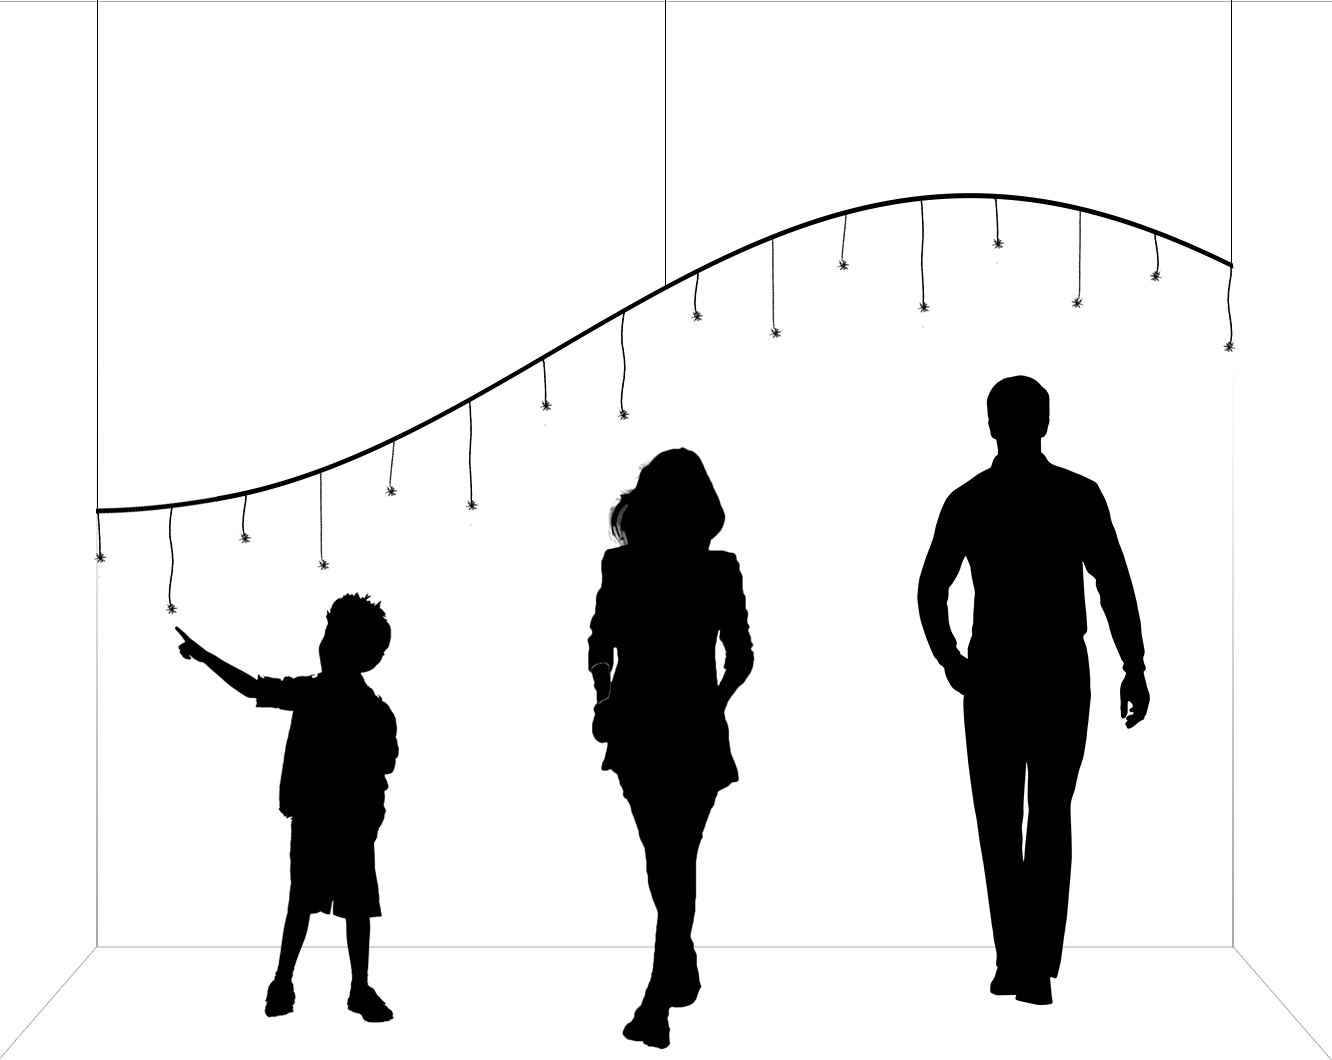
\includegraphics[width=0.8\textwidth]{./04-figuras/malha_futuro}
    \label{fig:malha_futuro}
  \end{center}
  \vspace*{-0,9cm}
  \fonte{Elaborada pela autora}\\
\end{figure}

Outro caminho natural diz respeito a aplicação e otimização de efeitos. Através de alteração do \textit{script} e utilização de portas analógicas seria possível, por exemplo, controlar a intensidade dos LEDs de acordo com a distância do espectador, fazendo-os acender ou apagar gradualmente à medida que o interator se afasta ou se aproxima. Além disso, também poderia ser estudada a manipulação de cores distintas através da utilização de LEDs RGB, neste caso, as possibilidades de variação dentro do mesmo trabalho são infinitas.

